\documentclass[10pt, usenames, dvipsnames, table]{beamer}
\usetheme{Berkeley}
\usecolortheme{seagull}
\usepackage{graphicx}
\graphicspath{ {../images/} }
\usepackage{array}
\RequirePackage{fix-cm}
\usepackage{colortbl}
\usepackage{hyperref}
\usepackage{graphbox}
\usepackage{algorithm}
\usepackage{algpseudocode}
\usepackage{minted}
\setminted{} % numbers=right, bgcolor=lightgray}


\title{The Scala Programming Language}
\author{Troy Hut and Benjamin Killeen}
\date{}

\begin{document}

\begin{frame}
  \titlepage{}
\end{frame}

\section{Introduction}
\begin{frame}
  \frametitle{Introduction}
  Scala is:
  \begin{itemize}
  \item<2-> Object oriented
  \item<3-> Functional
  \item<4-> Frustratingly well-typed
  \end{itemize}
\end{frame}

\begin{frame}
  \frametitle{Scala is \textbf{Scalable}}
  \begin{figure}
    \centering
    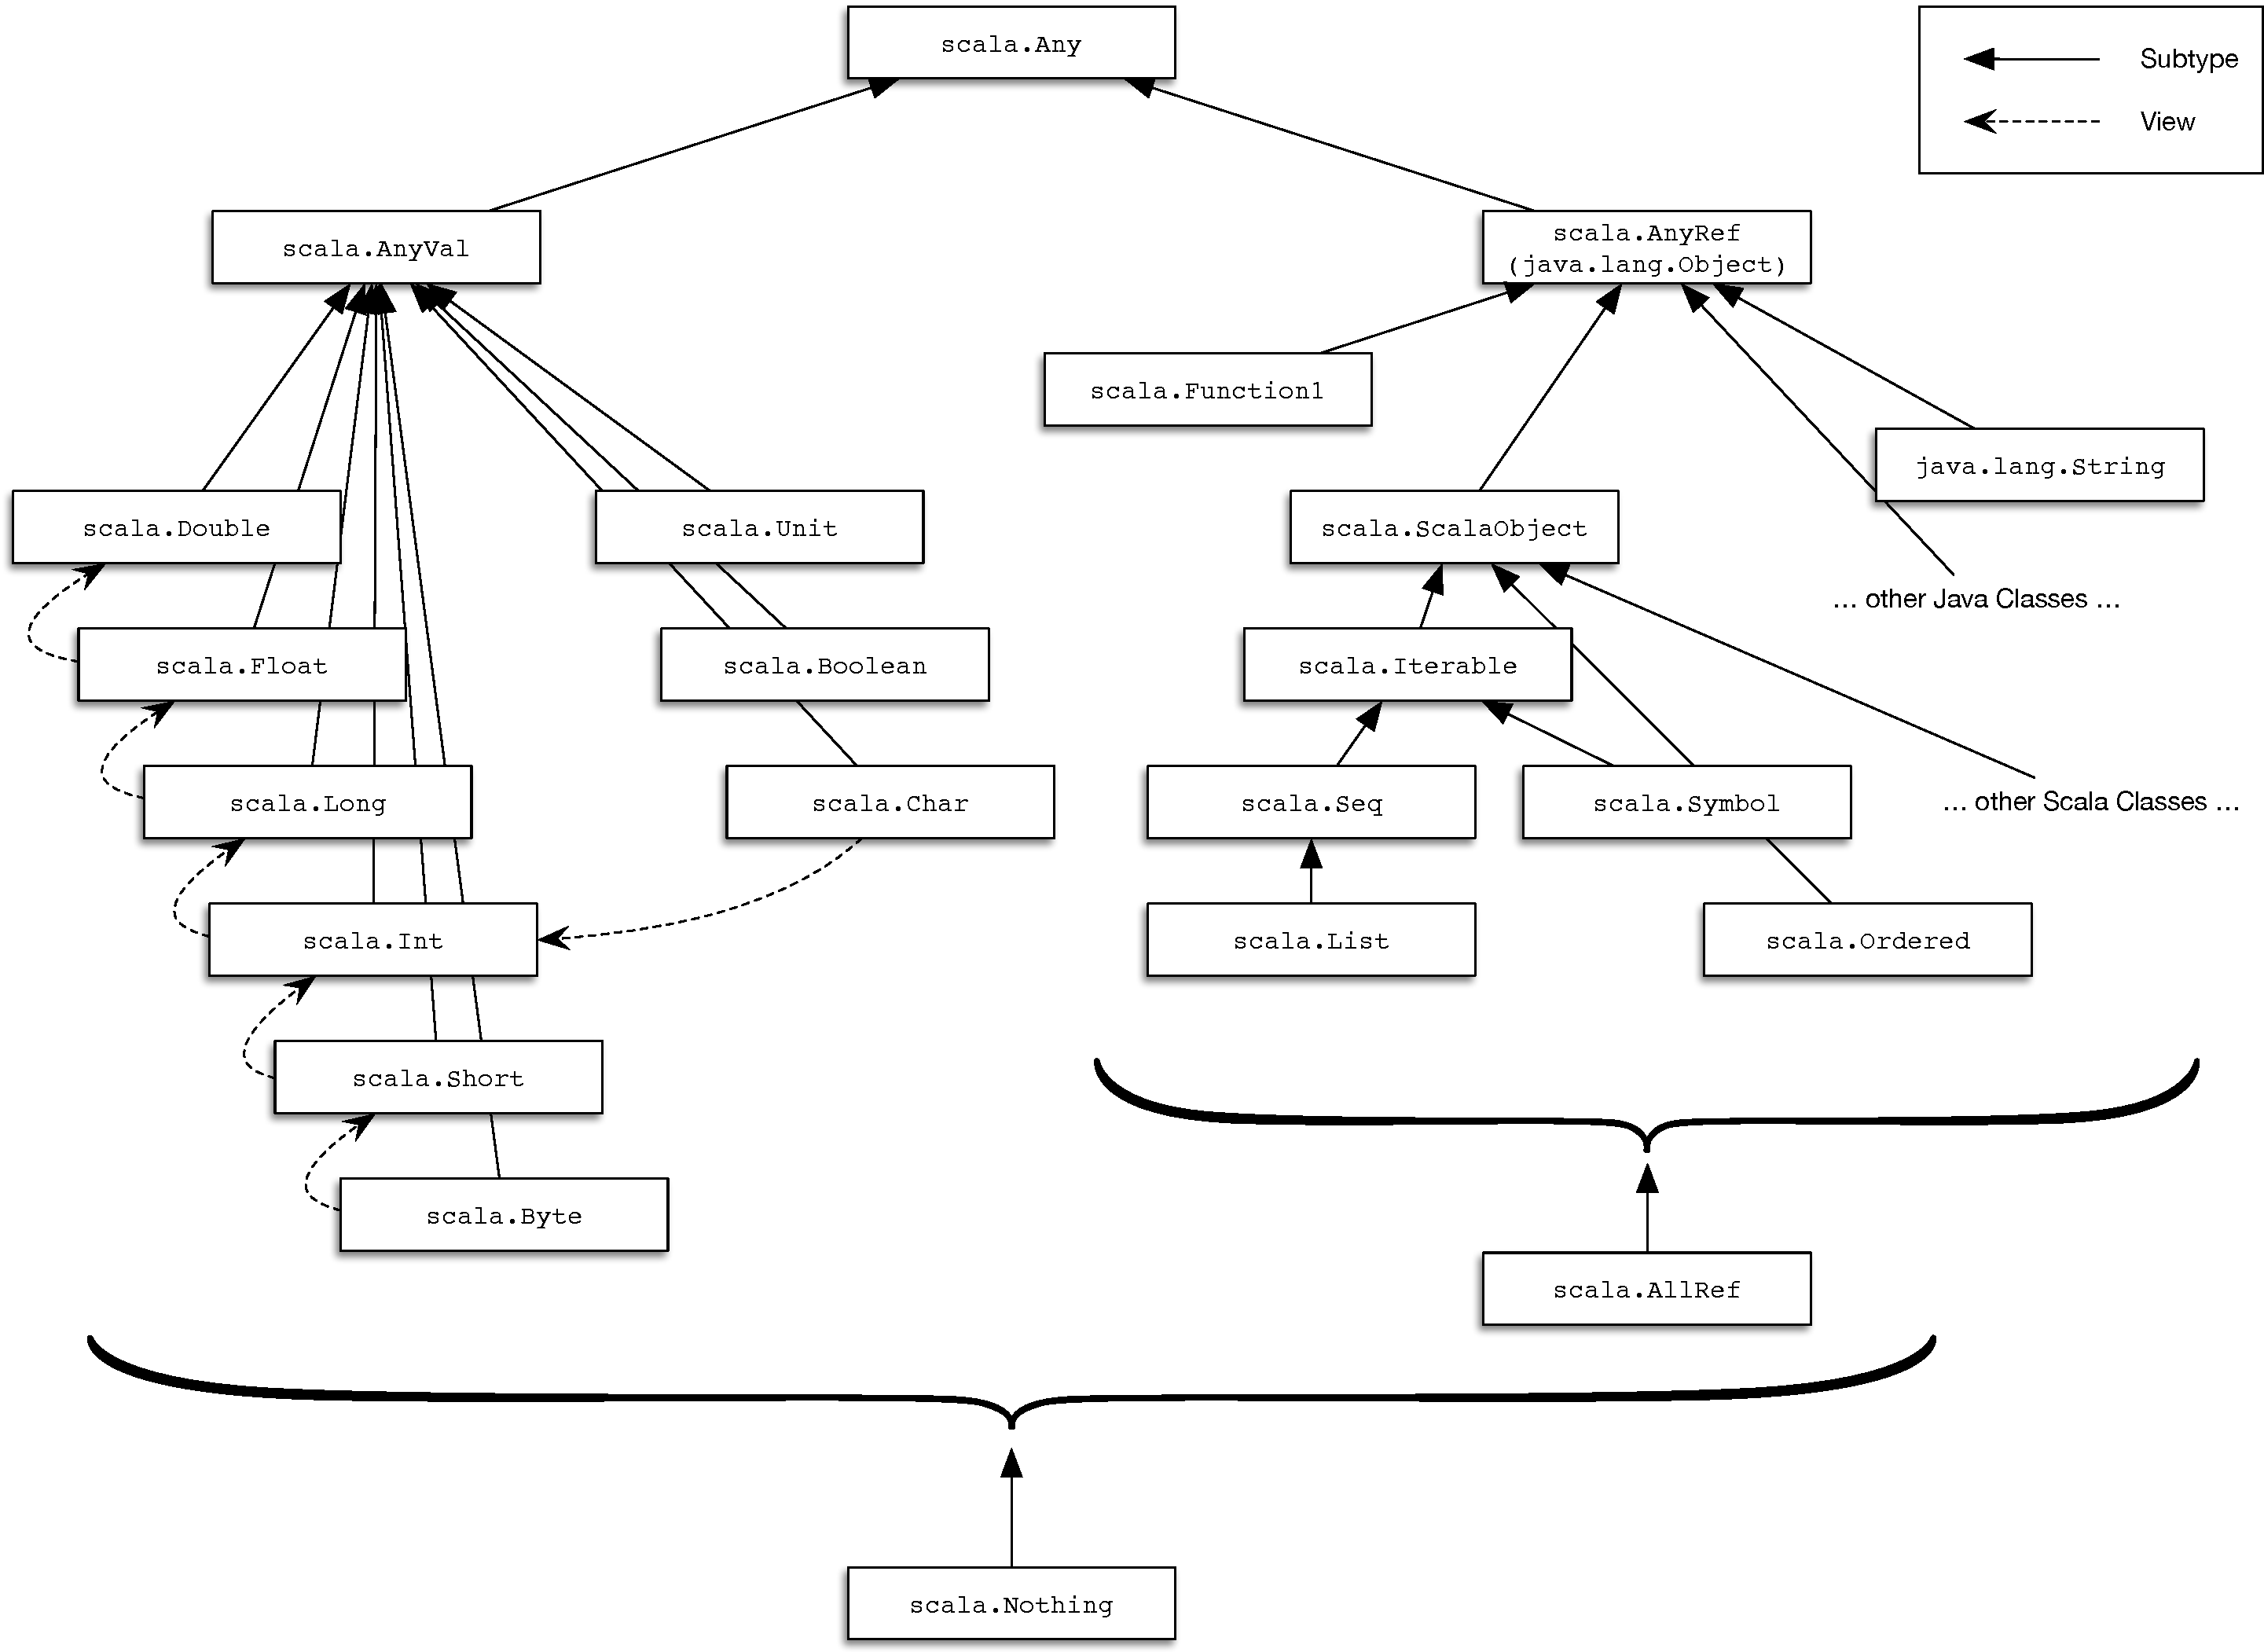
\includegraphics[width=0.8\linewidth]{scala_classes}
    \caption{The Scala class hierarchy.}
    \label{fig:class_hierarchy}
  \end{figure}
\end{frame}

\begin{frame}
  \frametitle{Traits, Objects, and Classes}
  \inputminted{Scala}{../examples/ExampleNat.scala}
  \pause{}
  \inputminted{Scala}{../examples/ExampleZero.scala}
  \pause{}
  \inputminted{Scala}{../examples/ExampleSucc.scala}  
\end{frame}

\begin{frame}
  \frametitle{Inferred Methods}
  \inputminted[firstline=1, lastline=1, fontsize=\tiny]
  {Scala}{../examples/Nat.scala}
  \inputminted[firstline=5, lastline=12, fontsize=\tiny]
  {Scala}{../examples/Nat.scala}
  \inputminted[firstline=19, lastline=19, fontsize=\tiny]
  {Scala}{../examples/Nat.scala}
  \pause{}
  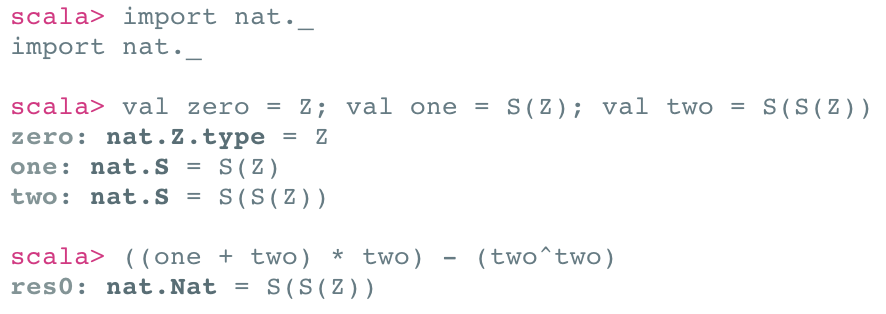
\includegraphics[width=0.7\linewidth]{nat_usage}
\end{frame}

\begin{frame}
  \frametitle{Type Parameters}
  \inputminted[fontsize=\small]{Scala}{../examples/Ord.scala}
\end{frame}

\begin{frame}
  \frametitle{The \mintinline{Scala}|nat| Package}
  \inputminted[firstline=1, lastline=28, fontsize=\tiny]
  {Scala}{../examples/Nat.scala}
  \vspace{-0.25\linewidth}
  \pause{}
  \flushright{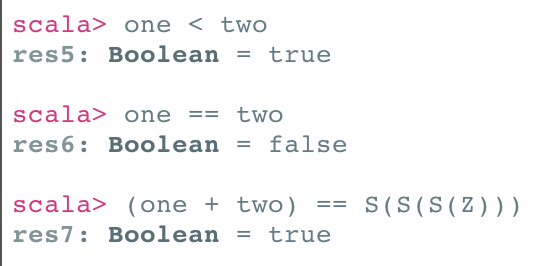
\includegraphics[width=0.4\linewidth]{nat_ordering_usage}}
\end{frame}

\begin{frame}
  \frametitle{Variance}
  \begin{block}{Covariance}
    If \mintinline{Scala}|C| is a \emph{covariant} type constructor and
    \mintinline{Scala}|S <: T|, then \mintinline{Scala}|C[S] <: C[T]|.
  \end{block}
  \pause{}
  \begin{block}{Contravariance}
    If \mintinline{Scala}|C| is a \emph{contravariant} type constructor and
    \mintinline{Scala}|S <: T|, then \mintinline{Scala}|C[S] >: C[T]|.
  \end{block}
\end{frame}

\subsection{Ordered List}
\begin{frame}
  \frametitle{Ordered List}
  \inputminted[firstline=1, fontsize=\tiny]
  {Scala}{../examples/OrdList.scala}
\end{frame}

\end{document}
%%% Local Variables:
%%% mode: latex
%%% TeX-master: t
%%% TeX-command-extra-options: "-shell-escape"
%%% End:
